\section{Zigbee}

Zigbee is a widely used wireless communication technology designed for low-power, low-data-rate applications. 
Its main features include:
\begin{itemize}
    \item \textit{Low-cost hardware and software}: devices typically cost around \$2, making Zigbee an affordable option.
    \item \textit{Short transmission range}: around 10 meters, which is suitable for local communication.
    \item \textit{Low latency}: ensures quick response times.
    \item \textit{High energy efficiency}: optimized for battery-powered devices, making it ideal for IoT applications.
\end{itemize}

\paragraph*{History}
In the mid-1990s, IoT solutions were highly fragmented, with numerous proprietary protocols leading to major compatibility and interoperability challenges. 
This also drove up costs, making large-scale adoption difficult.
To address this, IEEE launched Working Group 4 in 2001 to develop a standardized reference technology. 
This effort resulted in the IEEE 802.15.4 standard, which was officially published in March 2003.

Zigbee communication stack is composed as follows.
\begin{figure}[H]
    \centering
    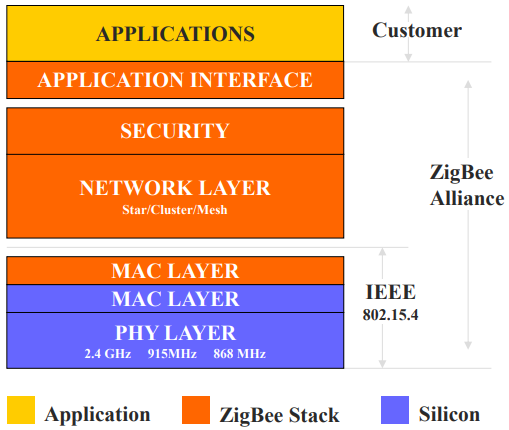
\includegraphics[width=0.5\linewidth]{images/zig.png}
    \caption{Zigbee communication stack}
\end{figure}

\paragraph*{Devices}
Zigbee networks consist of different types of devices, each playing a specific role:
\begin{itemize}
    \item \textit{Full function device}: can send beacons to manage network communication, communicate with other FFDs, route network frames, and act as a PAN coordinator. 
        Typically powered by an external power supply.
    \item \textit{Reduced function device}: cannot route frames or communicate with other RFDs.
        Communicates only with an FFD.
        Designed for low-power, battery-operated applications.
    \item \textit{PAN coordinator}: handles device association and de-association.
\end{itemize}

\paragraph*{Network topologies}
Zigbee networks support three different topologies, each suited for specific use cases:
\begin{itemize}
    \item \textit{Star topology}: all devices connect to a central coordinator.
        Simple, but limited in scalability.
        Common in home automation and industrial monitoring.
    \item \textit{Mesh topology}: devices communicate with multiple neighboring nodes.
        Highly reliable and scalable, as data can take multiple paths.
        Used in large-scale IoT deployments.
    \item \textit{Cluster-tree topology}: an hybrid between star and mesh.
        Devices are organized in clusters, with a coordinator managing each cluster.
        Efficient for applications requiring structured hierarchies, such as industrial automation.
\end{itemize}

\subsection{Physical layer}
The physical layer (PHY) of Zigbee, based on IEEE 802.15.4, is responsible for managing radio communication and ensuring reliable data transmission. 
Its main functions include:
\begin{itemize}
    \item \textit{Radio transceiver control}: activates and deactivates the radio module as needed.
    \item \textit{Energy Detection}: measures signal strength within the current channel, useful for scanning and channel selection.
    \item \textit{Link Quality Indicator}: evaluates the quality of received packets.
    \item \textit{Clear Channel Assessment}: determines if a channel is free before transmitting, enabling Carrier Sense Multiple Access with Collision Avoidance.
    \item \textit{Channel frequency selection}: supports multiple frequency bands to reduce interference.
    \item \textit{Data transmission and reception}: handles the actual exchange of data between devices
\end{itemize}
\noindent Zigbee operates across multiple frequency bands, offering flexibility based on regional regulations and application requirements: 868 MHz, 915 MHz, and 2.4 GHz. 

\paragraph*{Packet}
The physical layer defines the structure of transmitted data packets, ensuring synchronization and proper interpretation of information. 
The key components of a PDU (Packet Data Unit) are:
\begin{itemize}
    \item \textit{Preamble}: helps receivers synchronize with the incoming signal.
    \item \textit{Start frame delimiter} (SFD): marks the beginning of a valid frame.
    \item \textit{Frame length}: specifies the size of the PHY payload (in octets).
        For MAC data frames, the payload length ranges between 9 and 127 octets.
\end{itemize}

\subsection{Medium Access Control layer}
The MAC sublayer in IEEE 802.15.4 plays a crucial role in managing communication between devices in a Zigbee network. 
It provides key functionalities such as:
\begin{itemize}
    \item \textit{Beacon management}: synchronizes devices and schedules transmissions.
    \item \textit{Channel access management}: determines how devices share the communication medium.
    \item \textit{Guaranteed Time Slot management}: allocates dedicated transmission slots for time-sensitive data.
    \item \textit{Frame validation}: ensures data integrity and discards invalid frames.
    \item \textit{Acknowledged frame delivery}: confirms successful message reception.
    \item \textit{Association and disassociation}: manages device connections within a network.
    \item \textit{Security hooks}: provides mechanisms for implementing encryption and authentication.
\end{itemize}
\noindent Zigbee defines two operation modes to balance power efficiency and communication reliability:
\begin{enumerate}
    \item \textit{Beacon-enabled mode}: the PAN Coordinator periodically transmits beacons to synchronize devices.
        Commonly used in star topologies.
        Uses a combination of slotted CSMA-CA and scheduled transmissions to manage channel access.
    \item \textit{Non beacon-enabled mode}: devices communicate using unslotted CSMA-CA, meaning no predefined transmission schedule.
        Provides uncoordinated access, reducing overhead but increasing the risk of collisions.
\end{enumerate}

\paragraph*{Channel access mechanism}
Since multiple devices share the same frequency, Zigbee uses a mix of scheduled and random access to prevent interference:
\begin{itemize}
    \item \textit{Scheduled Access}: managed by the PAN Coordinator (only in beacon-enabled mode).
    \item \textit{Random Access}: used for communication between RFDs or between RFD/FFD and the PAN Coordinator.
        Allowed in both operation modes.
\end{itemize}

\paragraph*{CSMA-CA}
Zigbee devices rely on CSMA/CA to reduce transmission conflicts. 
Each device tracks key variables to manage communication: the number of backoffs, which counts transmission delays; the contention window, controlling how long the channel must remain clear before transmission; and the backoff exponent, determining the wait time before attempting access.
The CSMA/CA process begins with the transmitting node waiting for a random backoff period. 
If the channel remains clear for the required CW duration, the device proceeds with transmission and awaits an acknowledgment. 
However, if the channel is busy, the node increases both BE and NB, repeating the process until either a successful transmission occurs or the retry limit is reached, at which point the packet is discarded.
Additional factors influence this process. 
All transmissions, including ACKs, must complete within the Contention Access Period. 
While slotted CSMA/CA requires synchronization, unslotted CSMA/CA operates without it. 
Certain packets, such as beacons and ACKs, bypass CSMA entirely and transmit immediately. 
If a collision occurs—evident when no ACK is received—the device restarts the procedure.

\paragraph*{Network formation}
To join a network, Zigbee devices scan for available PANs. 
Active scanning, used by full-function devices, involves sending a beacon request, prompting nearby PAN coordinators to respond with beacons. 
After scanning, the device selects a PAN ID and joins. 
Passive scanning, available to both FFDs and reduced-function devices, operates similarly but without actively requesting beacons.
Instead, the device listens for beacon transmissions from coordinators.

\paragraph*{Extensions}
Enhancements to the IEEE 802.15.4 standard have expanded Zigbee's capabilities for specialized applications.
IEEE 802.15.4e introduces slotted channel access for improved efficiency. 
IEEE 802.15.4g targets smart utility applications, such as smart meters, while IEEE 802.15.4k optimizes communication for critical infrastructure monitoring, including power grids and industrial control systems.

\subsection{Network layer}
The network layer provides the following key functionalities:
\begin{itemize}
    \item \textit{Configuring a new device}: this involves setting up the device and configuring the stack to operate as required.
    \item \textit{Starting a network}: establishing a new network from scratch.
    \item \textit{Joining, rejoining, and leaving a network}: devices can join, rejoin, or leave a network. ZigBee coordinators or routers can also request devices to leave the network.
    \item \textit{Addressing}: ZigBee coordinators and routers have the responsibility of assigning unique addresses to devices joining the network.
    \item \textit{Neighbor discovery}: the ability to discover and report information about the device's one-hop neighbors.
    \item \textit{Route discovery}: the process of finding and recording paths within the network, allowing messages to be routed efficiently.
    \item \textit{Reception control}: the device can manage when the receiver is activated and for how long, supporting MAC synchronization and direct reception.
    \item \textit{Routing}: this encompasses various routing mechanisms, such as unicast, broadcast, multicast, and many-to-one, to efficiently exchange data within the network.
\end{itemize}
\noindent In ZigBee, there are three types of devices:
\begin{itemize}
    \item \textit{ZB coordinator} (FFD): the central coordinator that initiates and manages the network.
    \item \textit{ZB router} (FFD): routers that relay messages and allow other devices to join the network.
    \item \textit{ZB end-device} (RFD or FFD): end devices, which may either be reduced-function devices (RFDs) or full-function devices (FFDs).
\end{itemize}
\noindent ZigBee routing integrates two primary protocols: ad-hoc on-demand distance vector and cluster tree algorithm. 

\subsubsection{Cluster tree algorithm}
The Cluster Tree Algorithm defines how a ZigBee network organizes itself into a tree structure for efficient data routing.
The most important operations are: 
\begin{itemize}
    \item \textit{Tree initialization by FFD}: a ZigBee Full-Function Device (FFD) begins the tree formation by scanning available channels and selecting one with minimal interference. 
        It sets its PAN identifier and assigns itself the network address 0, indicating its role as the coordinator.
    \item \textit{Association of devices}: other devices can then join the network by associating with the coordinator through standard association procedures. 
        These devices may include routers (only FFDs) and end-devices.
    \item \textit{Address assignment}: during the association process, devices are assigned 16-bit short addresses. 
        The parent device (either the PAN coordinator or a ZB router) assigns address ranges to its child devices. 
        Each router receives a consecutive block of addresses based on its depth in the tree, while the first address in this block is used as the node's address, and the remaining addresses are available for its child devices.
        Address assignment follows a hierarchical structure. 
        The size of the address range $A(d)$ assigned to a router node at depth is calculated using the following formula:
        \[A(d)=\begin{cases} 1+D_m+R_m\qquad\text{if }d=L_m-1 \\ 1+D_m+R_mA(d+1)\qquad\text{if }0 \leq d <L_m-1 \end{cases}\]
        For each device, addresses are assigned in a range determined by its depth in the tree. 
        Devices further from the coordinator receive a larger range of addresses for their child devices.
    \item \textit{Coordinator constraints}: the ZigBee coordinator also defines key network parameters, such as the maximum number of routers ($R_m$) and end-devices ($D_m$) each router can support, as well as the maximum depth ($L_m$) of the tree.
\end{itemize}

\paragraph*{Tree routing}
Routing within a ZigBee network follows the tree structure formed by the coordinator and its child devices. 
Messages are routed through the tree in the following manner:
\begin{itemize}
    \item If the destination address belongs to one of the child end-devices, the message is routed directly to the destination.
    \item If the destination address corresponds to a child router, the message is sent to that router for further forwarding.
    \item If the destination address is not found among the children, the message is forwarded to the parent node for further routing.
\end{itemize}
This tree-based routing system is simple and works efficiently, although it may not always provide the most optimized routes. 
It is also quality-agnostic, meaning the routing decisions do not take into account the quality of the link.

\subsubsection{Ad-hoc on demand distance vector}
In contrast to tree routing, Ad-hoc On-demand Distance Vector (AODV) is a reactive routing protocol used when a device needs to send data to an unknown destination. 
Here's how AODV works:
\begin{enumerate}
    \item \textit{Route request} (RREQ): when a device wants to communicate with a destination, it broadcasts a Route Request (RREQ) message.
    \item \textit{Flooding}: the RREQ message is flooded across the network, and each node that relays the request stores the address of the node that forwarded it, setting up a reverse path to the source.
    \item \textit{Route reply} (RREP): when the destination node receives the RREQ, it sends a Route Reply (RREP) message back to the source, traveling along the reverse path set up during the flooding process.
\end{enumerate}
\noindent Routing tables are updated as nodes process these RREQ and RREP messages. 
A node's routing table contains the following entries:
\begin{itemize}
    \item \textit{Destination address}: the address of the destination.
    \item \textit{Next-hop address}: the address of the next hop toward the destination.
    \item \textit{Entry status}: whether the entry is active, in discovery, or inactive.
\end{itemize}
\noindent Additionally, a Routing Discovery Table (RDT) keeps track of RREQ messages, storing information like the source address, the sender's address, and the accumulated path cost.

\paragraph*{Routing cost}
The cost of a path $P$ is the sum of the individual costs of the links that make up the path. 
The cost for each link $l$ is determined by factors like the packet reception rate $p_l$ and follows a standard cost function, which suggests a value of 7 for a link with poor reception and a function based on the reception rate for links with better performance: 
\[C(l)=\begin{cases}
    7 \\ 
    \min\left(7,\text{round}\left(\dfrac{1}{p_l^4}\right)\right)
\end{cases}\]

\paragraph*{Application profiles}
ZigBee also provides predefined application profiles that ensure interoperability across different devices and manufacturers. 
These profiles define the following:
\begin{itemize}
    \item A common language for data exchange.
    \item A well-defined set of processing actions for devices.
    \item Device interoperability across manufacturers.
    \item Simplicity and reliability for end users.
\end{itemize}
\noindent Each profile is made up of:
\begin{itemize}
    \item A set of devices needed for the application.
    \item A set of clusters that implement the required functionality.
    \item A set of attributes representing device state.
    \item A set of commands enabling communication between devices.
\end{itemize}